
\label{chapter:fund_teo}
Este capítulo tem como objetivo apresentar os conceitos e definições abordados neste trabalho, tais como: Sistemas Embarcados, Modelos Formais para Verificação de Sistemas, Visão Computacional e Reconhecimento de Padrões.
  
    
    
\section{Sistemas Embarcados} 

Sistemas computacionais estão por toda parte e muitos deles estão em computadores pessoais, já sistemas embarcados são um tipo específico de sistema computacional que pode ser encontrado em uma grande gama de dispositivos, desde \textit{notebooks, tablets} a jogos eletrônicos portáteis, máquinas de fax, entre outras coisas como eletrodomésticos~\cite{vahid:2002}.

Segundo~\citeonline{vahid:2002}, um sistema embarcado é qualquer sistema computacional que não seja um computador pessoal ou \textit{workstation}. \citeonline{heath:2002} define sistemas embarcados como sistemas baseados em microprocessadores ou microcontroladores (ver Seção~\ref{Sect:Micros}), construídos para executar uma \textbf{função específica} ou grupos de funções programadas. Os sistemas embarcados não são projetados para serem reprogramados da mesma forma que computadores pessoais.
% 
Um dos exemplos citados por \cite{heath:2002} como sistema embarcado é uma máquina de lavar, que possui vários ciclos de lavagem, painéis para acompanhar os ciclos e controle dos motores, e bombas de água.


Já \citeonline{schlett:1998} diz que um sistema embarcado precisa executar uma tarefa específica com o menor custo energético e monetário possível.
%O custo energético é um dos grandes desafios encontrados no desenvolvimento de sistemas embarcados.
Neste sentido, segundo \citeonline{vahid:2002}, algumas características de sistemas embarcados são:\begin{itemize}
\item Função única: Sistemas que são programados para um tarefa específica, que pode se repetir várias vezes.
\item Fortemente limitado: Sistema com limitações definidas nas suas métricas de projeto, como de desempenho, consumo de energia, preço e dimensões.
\end{itemize}


\todo[inline]{Descrever como os SE tem impactado os dias atuais, Exemplificar}
 

% =========================================================
\subsection{Microcontroladores x Microprocessadores}
\label{Sect:Micros}
% =========================================================        

Os computadores modernos são baseados em microprocessadores\todo{apresentar exemplo com referência}, permitindo-os realizar várias funções, enquanto outros sistemas baseados em microcontroladores, são limitados a apenas um ciclo repetido da mesma tarefa~\cite{heath:2002}. Microcontroladores são compostos por vários componentes integrados a ele, como RAM, interface de entrada e saída e uma memória re-programável~\cite{white:2011}.

%Segundo \citeonline{white:2011} define microcontroladores como processadores com componentes atrelados a ele, com memória re-programável

Sistemas embarcados derivaram de processadores desenvolvidos para o mercado de computadores domésticos, com algumas diferenças no consumo energético, preço e componentes atrelados à CPU. Outras diferenças são o tempo de resposta de interrupções, a quantidade de memória e portas paralelas \cite{schlett:1998}.


As vantagens de um microcontrolador são mobilidade, baixo consumo de energia, custo, segurança e confiabilidade, uma vez que sistemas embarcados são sistemas 
% modestos, 
altamente otimizados usualmente com baixo poder de processamento, realizando tarefas de extremo risco\todo{descrever} em tempo real. Por outro lado computadores baseados em microprocessadores possuem alto poder de processamento, por um alto custo, tanto energético quanto monetário. %informações do slide, irei citar)

Um exemplo de um sistema baseado em microcontrolador é o \textit{Arduino Uno} \cite{Arduino2018ArduinoRev3} que é uma microcontrolador que possui $14$ pinos digitais, $6$ portas analógicas, cristal de quartzo com frequência de $16$Mhz, conexão USB e entrada de alimentação eletrica. O \textit{Arduino} pode ser reescrito várias vezes utilizando um computador e no pior dos casos você pode substituir o microcontrolador com um preço acessível.

\todo[inline]{Ampliar a descrição sobre o Arduino}

Existem também os \textit{Single Board Computers}, um bom exemplo é o \textit{Raspberry PI}, que segundo \citeonline{Pi2016DATASHEETCM3L}, possuem processador e memória integrados, os caracterizando como microcontroladores ou modulo computacional. As vantagens da utilização são por seu baixo custo, baixo consumo energético e alta rentabilidade e grande quantidade de portas para uso geral como pode ser visto no \textit{datasheet} da \autoref{fig:raspsheet}.
 \begin{figure}[H]
	\centering
    	\caption{\label{fig:raspsheet} CM3/CM3L Diagrama }
		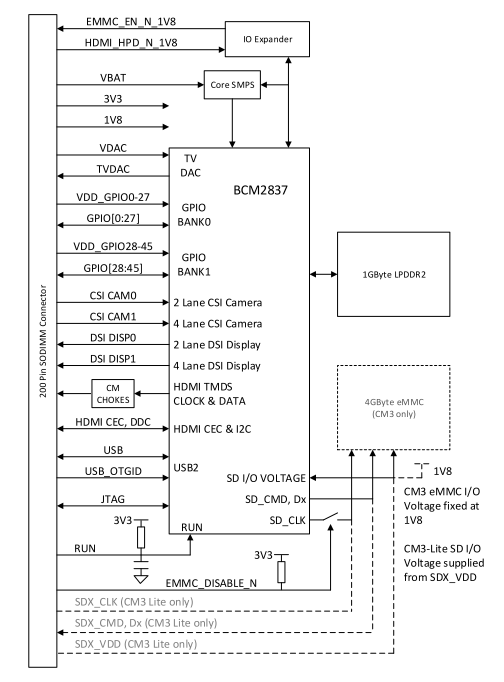
\includegraphics[width = 0.8\textwidth]	{resources/raspsheet}
    	\legend{Fonte: \cite{Pi2016DATASHEETCM3L}}
\end{figure}

\todo[inline]{Apresentar exemplos de uso na prática com Raspberry PI}

\todo[inline]{Apresentar um discussão de quando usar Microcontroladores ou Single Board Computers com Microprocessadores}


% =========================================================
\subsection{Internet das Coisas(IoT - Internet of Things)}
% =========================================================

A Internet das Coisas (IoT - \textit{Internet of Things}) é paradigma que está ganhando espaço no cenário moderno de telecomunicações sem fio. Sendo seu conceito básico conectar uma vasta quantidade de coisas ou objetos (casas, carros, sinais de trânsito e outros), fazendo-os interagir entre si para alcançar um objetivo em comum \cite{atzori2010internet}.


Segundo \cite{xia:2012} a Internet das Coisas é um conceito que interligará todos os dispositivos através de sistemas embarcados, formando uma rede de dados inteligente, ubíqua e distribuída. Os dispositivos podem trazer avanços que irão melhorar a qualidade de vida, facilitando a comunicação entre pessoas e dispositivos.

Todos os dispositivos ao nosso redor estarão conectados a internet, isso resultará numa enorme quantidade de dados que terão de ser processados e apresentados sem falhas de forma eficiente. A computação em nuvem pode oferecer uma infraestrutura de ponta a ponta, entre o dispositivo e o servidor satisfazendo essa demanda de qualquer lugar \cite{Gubbi:2013}.

Internet das Coisas é sobre ampliar o escopo de conexões para objetos que não são convencionais de estarem conectados à rede. Por esse motivo uma grande quantidade de soluções de comunicação foram introduzidas, visando o melhor custo energético \cite{siekkinen2012low}. 
% E a utilização dessa visão neste trabalho será onde 

Na tentativa da caracterização da Internet das Coisas, A \autoref{fig:iotoverview} coloca os principais conceitos, tecnologias e padrões na visão desse paradigma, destacando e classificando as diferentes visões que resultam na Internet das Coisas, mostrando o melhor resultado de uma convergência.

 \begin{figure}[H]
	\centering
    	\caption{\label{fig:iotoverview} Paradigma "Internet das Coisas" (IoT) como resultado da convergência de diferentes visões }
		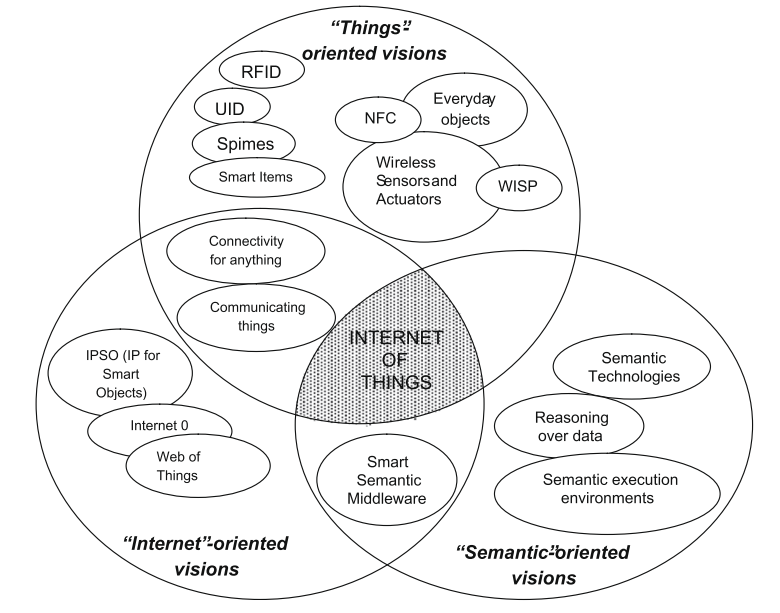
\includegraphics[width = 0.8\textwidth]	{resources/iotoverview}
    	\legend{Fonte: \cite{atzori2010internet}}
\end{figure}

\todo[inline]{Apresentar um exemplo detalhado de IoT}


% =========================================================
\subsection{Baixo consumo de energia}
% =========================================================

Os dispositivos que compõem a Internet das Coisas são caracterizadas por utilizar poucos recursos, em termos de computação e capacidade energética. Isso requer certa atenção, já que novos projetos terão que levar em consideração à eficiência dos recursos e problemas de escalabilidade \cite{atzori2010internet}.

Com o avanço da Internet das Coisas, uma grande demanda de dados surgiu e por sua vez a alocação e gerenciamento de dados se tornaram um problema crítico. Atualmente a internet utiliza 5\% da energia gerada com a solução desses tipos de problemas, e tende a crescer cada vez mais~\cite{Gubbi:2013}.

Geralmente há restrições no \textit{hardware} e \textit{software}\todo{Apresentar exemplos}. As restrições de \textit{hardware} ajudam a limitar a utilização de recursos energéticos e monetários, e as de \textit{software} limitam o programa a um determinado ciclo, podendo esse ser determinístico ou/e tempo real, reagindo de forma rápida e tolerante a falhas. Essas restrições são dadas pois um sistema embarcado faz parte de um sistema maior, muito mais composto. %informações do slide irei citar 19/01/18

\todo[inline]{Está seção está muito raza, explanar mais e apresentar um técnica para redução de consumo de energia}


% =========================================================
\section{Modelos formais para verificação de sistemas}
% =========================================================
%falar sobre verificação de sistemas. A importância e onde é usada. Falar sobre modelos formais. Falando que a seção fala sobre exemplos de modelos formais. 
 
De acordo com \citeonline{Baier:2008} sistemas de Tecnologia da Informação e Comunicação (TIC) estão crescendo rapidamente, e seu funcionamento de forma eficaz é fundamental. Esses sistemas estão se tornando cada vez mais complexos e estão ganhando espaço no cotidiano através da internet e de todos os tipos de sistemas embarcados. Sistemas TIC estão por toda parte, eles controlam a maioria dos dispositivos de uso cotidiano\todo{Apresenatar exemplos}.

A dependência do uso de sistemas embarcados tornam sua eficácia fundamental para sociedade. Esses sistemas oferecem um bom desempenho em tempo de resposta e capacidade de processamento. O mal funcionamento desses sistemas podem ameaçar nossas vidas, e podem ter consequências financeiras substanciais para o fabricante. Sistemas TIC eficazes são fundamentais para a sobrevivência de uma empresa.

\todo[inline]{Apresentar exemplo de um falha de SE com resultado critico}

O crescimento na complexidade dos sistemas TIC mostram que eles não estão mais isolados, agora podem fazem parte de um grande sistema, conectando e interagindo com vários outros outros componentes, tornando esses sistemas vulneráveis a erros. 
A concorrência e o não determinismo que são fundamentais para a modelagem dos sistemas integrados, tornando a utilização de técnicas padrões muito difícil.

Técnicas de verificação são aplicadas a sistemas TIC de forma mais confiável. A verificação de sistemas trabalha pra estabelecer que o produto possua certas propriedades, como certificar que o sistema não entre em uma situação de \textit{deadlock}. A falha é encontrada quando o sistema não cumpre todas as propriedades especificadas\todo{Adicionar referência}.


%\subsection{Máquina finita de Estados}
%yMáquina finita de estados é um automato que ajuda a demonstrar o fluxo de um sistema computacional. (pré-texto) 

% =========================================================
\subsection{UML}
% =========================================================

Segundo \citeonline{rumbaugh2017unified} UML (\textit{Unified Modeling Language)} é uma linguagem de modelagem visual que tem como intuito de utilizar todos os métodos de desenvolvimento de software, extraindo melhor para especificar, visualizar, desenvolver e documentar os artefatos de um sistema em nível de software, capturando estáticas informais e dinâmicas do comportamento de um sistema.

\todo[inline]{Descrever os tipos de diagramas das UML e o objetivo de cada um deles.}

A utilização de UML nesse trabalho se dará pela utilização de diagramas de sequência que mostrarão como o fluxo do software irã ocorrer. De acordo com \citeonline{rumbaugh2017unified}, diagramas de sequência mostram a iteração em uma forma bidimensional, onde o eixo vertical é o tempo de vida do processo e o eixo horizontal mostra as regras de transição como pode ser visto na Figura~\ref{fig:sequencerumbaugh}. %Essas regras são definidas pelas setas que são os processos do software.

\todo[inline]{Explicar a Figura~\ref{fig:sequencerumbaugh}}

Já \citeonline{Cunha2011FormalContext} diz que diagramas de sequência as ações são organizadas por tempo\todo{Corrigir esta frase}, mas não exploram as relação dos objetos. Os diagramas de sequência mostram todo o processo de trocas de mensagens dos objetos, mapeando todo o ambiente mostrando como os objetos colaboram entre si para obter sucesso. Um exemplo é a \autoref{fig:sequencerumbaugh}, que mostra um diagrama de sequencia, com ator, processos e ações que são executas em certa ordem. 
 \begin{figure}[H]
	\centering
    	\caption{\label{fig:sequencerumbaugh} Diagrama de sequência }
		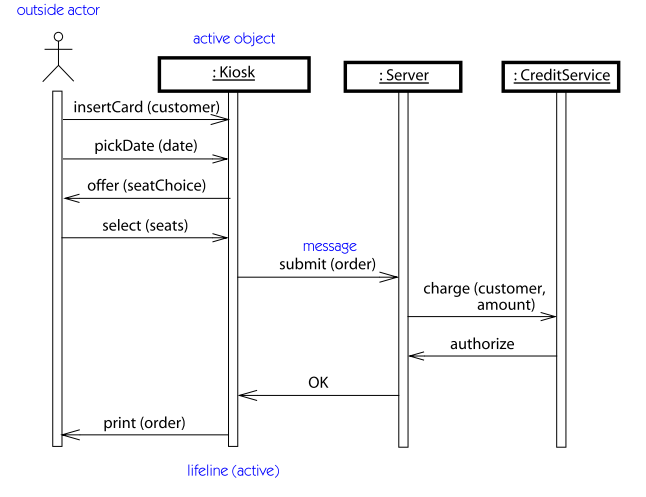
\includegraphics[width = 0.8\textwidth]	{resources/sequencediagramrumbaugh}
    	\legend{Fonte: \cite{rumbaugh2017unified}}
\end{figure}




%falar o que é. pra que é usado, e onde será usado no trabalho

% \todo{Computer vision is a vast fi eld. Th is book will give you a basic grounding in the fi eld, but we also recom- mend texts by Trucco [Trucco98] for a simple introduction, Forsyth [Forsyth03] as a comprehensive refer- ence, and Hartley [Hartley06] and Faugeras [Faugeras93] for how 3D vision really works}
% wa

\subsection{Redes de Petri}

Redes de Petri são modelos gráficos e matemáticos que podem ser aplicados em diversos sistemasa\todo{Exemplos}. Um método capaz de descrever e analisar as transições do sistema, podendo ele ser concorrente, assíncrono, distribuído, paralelo e não-determinístico. O modelo gráfico é capaz de auxiliar na visualização do fluxo, e a ferramenta matemática pode estruturar equações matemáticas para validação de propriedades formais do sistema analisado. O comportamento de sistemas pode ser descrito em estados, um estado em uma rede de Petri é alterado de acordo com a regra de transição~\cite{murata:1989}.

\todo[inline]{Apresentar a definição formal de uma RP.}

Segundo \citeonline{rumbaugh2017unified}, ainda que uma máquina de estados seja bem estruturada, um grupo de transições pode levar a sérias inconsistências, incluindo \textit{deadlocks} e outros problemas. Esses problemas foram bastante estudados na teoria das redes de Petri. 

 \begin{figure}[H]
	\centering
    	\caption{\label{fig:petri}Regra de transição}
		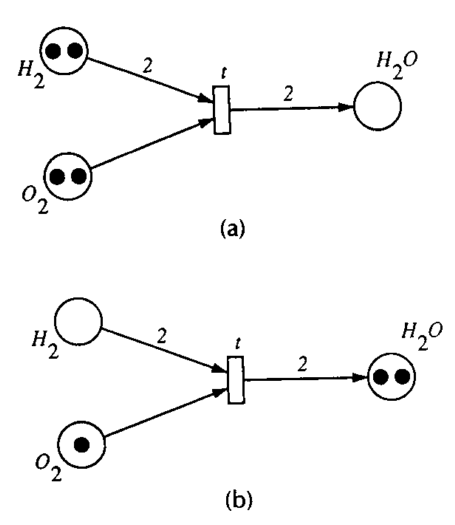
\includegraphics[width = 0.3\textwidth]	{resources/petri}
    	\legend{Regra de transição, (a) aceitação antes da transição \textbf{\textit{t}}. (b) iteração após aceitação de \textbf{\textit{t}}, \textbf{\textit{t}} está desativado.\cite{murata:1989}}
\end{figure}

\todo[inline]{Seção muito raza, explicar as propriedades de RP com exemplos, e então apresentar um exemplo prático tipo um semaforo.}

\section{Visão Computacional}

A visão humana não tem dificuldades em identificar pequenas variações na translucidez e sombreamento em imagens, distinguindo os objetos da imagem que é fundo. Temos certa facilidade em identificar estruturas tridimensionais, podemos diferenciar formatos, texturas, cores e pessoas em imagens, e até mesmo dizer que sentimentos eles podem estar sentindo, apenas olhando fotos \cite{szeliski2010computer}.
% 
A visão computacional é uma forma de emular a visão humana, possuindo imagens como entrada, e sua saída é a interpretação dessa imagem \cite{marengoni:2009}.

\citeonline{bradski:2008} definem uma parte da vasta área da visão computacional como uma transformação de dados de uma imagem em uma nova representação para atingir um objetivo específico, como deixar a imagem em escala de cinza. Essas transformações precisam de contexto, como especificar distância, referências de onde a imagem foi tirada, ou o que pode conter na imagem.
\begin{figure}[h]
	\caption{\label{fig:grayscaleex}Aplicação de uma equalização de histograma, em nível de cinza, onde a placa do veículo pode ser lida (direita).}
	\begin{center}
	    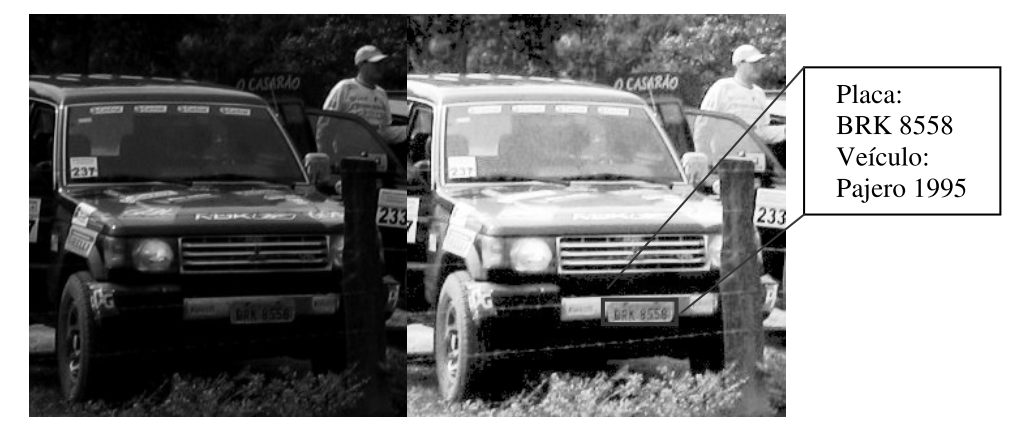
\includegraphics[width=.7\textwidth]{resources/grayscaleex}
	\end{center}
	\legend{Fonte: \cite{bradski:2008}}
\end{figure}


De acordo com \citeonline{marengoni:2009}, o processamento da imagem geralmente é a primeira etapa do processo de visão computacional, podendo ser dividido em três níveis: baixo-nível, nível-médio e alto-nível.
\begin{itemize}
\item Baixo-nível: 
	Pode ser associado a operações como redução de ruídos ou níveis de contraste da imagem. 
   \begin{figure}[h]
	\caption{\label{fig:blur}Aplicação de filtro Gaussiano para remoção de ruídos}
	\begin{center}
	    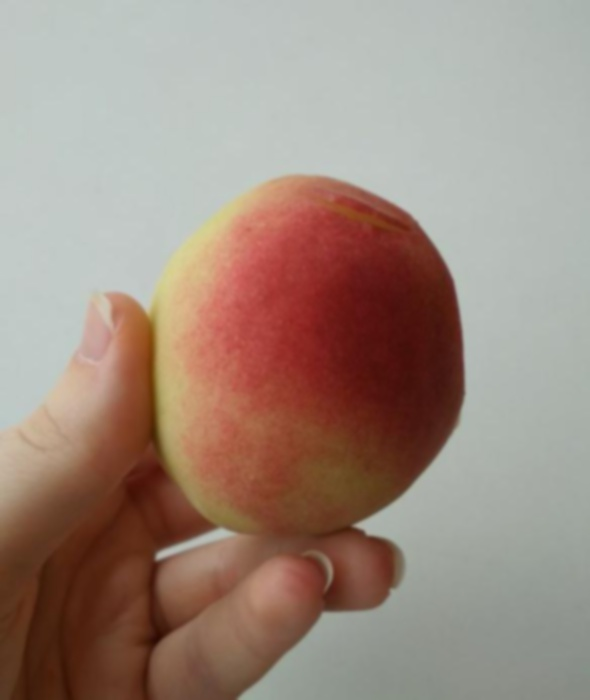
\includegraphics[width=0.3\textwidth]{peachs/blur}
	\end{center}
	\legend{Fonte Própria}
\end{figure} 
\item Nível-médio:
	São operações associadas a operações de segmentação de imagem ou reconhecimento de objetos na imagem.   
       \begin{figure}[H]
	\caption{\label{fig:segment}Segmentação com base nas cores da imagem com sobreposição para identificação de pêssegos.}
	\begin{center}
	    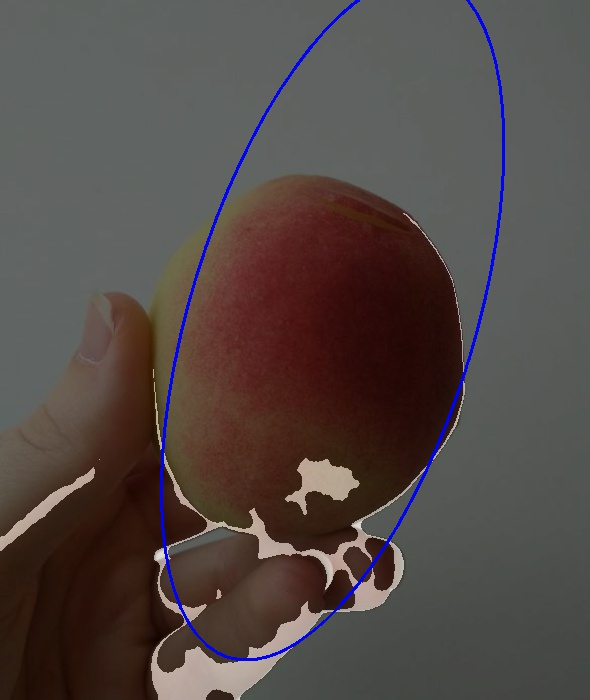
\includegraphics[width=0.3\textwidth]{peachs/identified}
	\end{center}
	\legend{Fonte Própria}
\end{figure}

\item Alto-nível:
São relacionados a tarefas de cognição associadas com a visão humana.
       \begin{figure}[h]
	\caption{\label{fig:machineflow}Identificação de objetos utilizando aprendizado de máquina.}
	\begin{center}
	    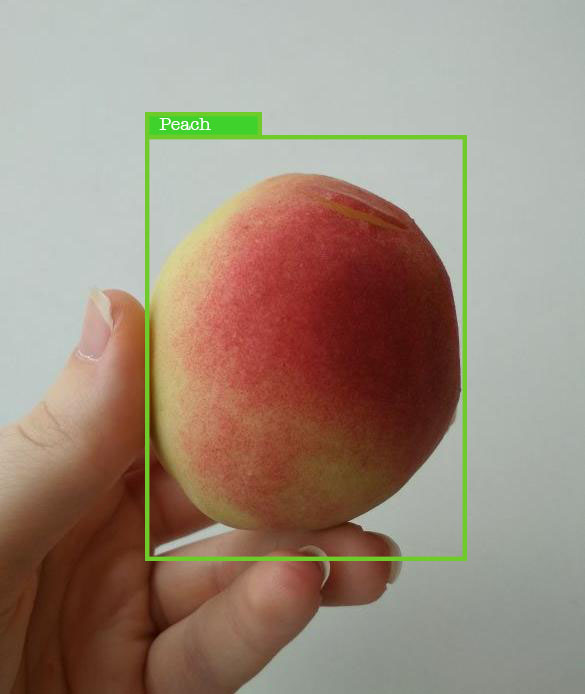
\includegraphics[width=0.3\textwidth]{peachs/tensorflow}
	\end{center}
	\legend{Fonte Própria}
\end{figure}
	
\end{itemize} 

% ----------------------------------------------
% ---------------------------------------------- 
\subsection{Representação de Imagens Digitais}
Uma imagem pode ser definida como uma função bidimensional, $f(x,y)$, onde $x$ e $y$ são coordenadas espaciais, e a amplitude de $f$ em qualquer par de coordenadas $(x,y)$ é chamada de intensidade da imagem, naquele determinado ponto. Quando $x,y$ e os valores de amplitude de $f$ são finitos, chamamos a imagem de imagem digital. Uma imagem digital é composta por um número finitos de elementos, cada um tendo seu próprio ponto e posição específicos. Esses elementos se referem à elementos de imagem, \textit{pels} e \textit{pixels} \cite{gonzalez1992digital}. 

O termo processamento de imagens digitais normalmente se referem ao processamento de imagens bidimensionais por computadores. Uma imagem digital é um vetor de números reais ou números complexos representados por uma quantidade finita de \textit{bits}.
Na representação de imagem devemos nos preocupar com a caracterização e quantidade de elementos que representam a imagem (\textit{pixels} ou \textit{pels}). Em geral qualquer função bidimensional que contém alguma informação pode ser considerada uma imagem. O principal requisito para o processamento de imagens digitais é que ela seja amostrada e logo em seguida quantificada. A taxa de amostragem, que são os \textit{pixels} por unidade de área, tem de ser grande o suficiente para preservar uma quantidade de informações úteis na imagem. A quantização da imagem é a conversão analógica para digital de uma imagem amostrada para um número finito de níveis de cinza \cite{jain1989fundamentals}.
 \begin{figure}[h]
	\caption{\label{fig:digitalproc}Típica sequência de processamento de imagem digital.}
	\begin{center}
	    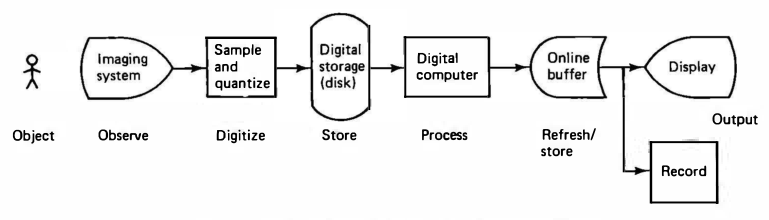
\includegraphics[width=.9\textwidth]{resources/digitalproc}
	\end{center}
	\legend{Fonte: \cite{jain1989fundamentals}}
\end{figure}


%\subsection{Pré-processamento de Imagem}

%\subsection{Segmentação e Detecção de Objetos}

%\subsection{Pós-Processamento}

\section{\textit{Frameworks} para identificação de imagem}
Nesta sessão iremos abordar \textit{frameworks} para identificação e classificação de imagens, onde são usando, as vantagens e desvantagens em  relação a métodos convencionais e tecnologias que utilizam \textit{frameworks} para suas atividades. %melhorar depois%

\todo{falar sobre aprendizado de máquina na sua utilização no projeto: como caixa preta}
%De acordo com \cite{papag} As dificuldades na identificação de objetos de interesse do mundo real, como rostos e pessoas são dadas pela complexidade desses tipos de objetos, uma quantidade significante de variedade de cores e texturas e o contraste com o fundo da imagem. Em comparação com a classificação de padrões, onde é necessário decidir entre classes bem definidas, na detecção de objetos é necessário diferenciar a classe de objeto para o que é o resto. 

\subsection{\textit{Tensorflow}}
Tensorflow é um \textit{framework} para operações computacionais, tendo uma grande biblioteca permitindo o desenvolvimento para diferentes plataformas, de \textit{clusters} de servidores até dispositivos móveis. Tensorflow tem grande facilidade de lidar com problemas de aprendizado de máquina e \textit{deep learning}, podendo ser usado em diversos domínios científicos \cite{tensorflow2015}. A utilização do \textit{framework} será de extrema importância nas classificações de imagens que serão processadas.



\subsection{YOLO}
\todo{fazer a mesma coisa pro YOLO (mesma coisa do tensorflow)}

%\section{Aprendizagem de máquina}
%Falar o que é. onde é usado, mostrar exemplos (muitas imagens), visão geral pra ter uma ideia do que é capaz

%\subsection{Redes Neurais}
%\todo{num sei}

%\subsection{Redes Neurais Convolutivas}
%\todo{num sei}

%\section{Reconhecimento de Padrões}


%\subsection{Aprendizado de máquina} 


%\subsection{Classificação de Padrões}


 
% \subsubsection{Homomorphic filtering} 
% 	O filtro homomórfico (\textit{homomorphic filter}) é um filtro de frequência usado para corrigir iluminações não uniformes e realçar o contraste na imagem processada \cite{bazeille2006}.
     
%  \begin{figure}[H]
% 	\centering
%     	\caption{\label{fig:homofilter}Homomorphic Filtering}
% 		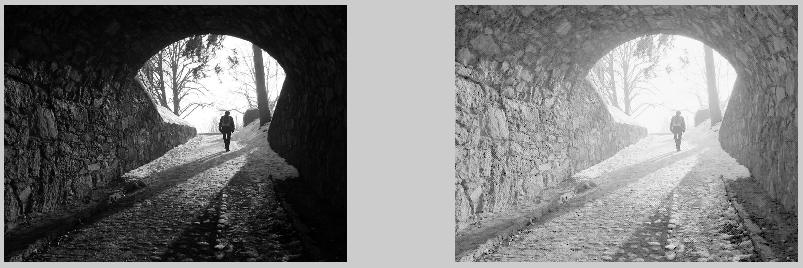
\includegraphics[width = 0.9\textwidth]	{resources/homofilter}
%     	\legend{\textit{Homomorphic filtering}, usando \textit{Butterworth High Pass Filter} para fazer a filtragem \cite{mathworks:2008}}.
% \end{figure}

%     %Considerando o modelo de reflectância, assumimos que uma imagem é o produto descrito pela equação:
%     \[
%     %	f (x,y) = i(x,y).r(x,y)
%     \]
%     %Sendo $f(x,y)$ é a imagem captada por um sensor ótico, $i(x,y)$ o fator multiplicativo de iluminação e $r(x,y)$ a função de reflectância. 
    

% \subsubsection{Anisotropic filtering}
% O Filtro anisotrópico permite a simplificação de atributos da imagem para melhorar a segmentação,  suavizando as partes homogêneas preservando as bordas e melhorando-as.

%  \begin{figure}[H]
% 	\centering
%     	\caption{\label{fig:anisifilter}Anisotropic Filtering}
% 		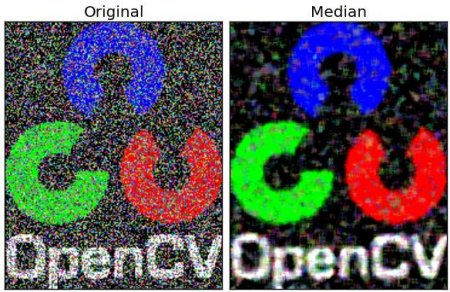
\includegraphics[width = 0.6\textwidth]	{resources/anisifilter}
%     	\legend{Fonte:\cite{mathworks:2008}}.
% % \end{figure}

% \subsection{Sensores de Aquisição de Imagens}
% Segundo \citeonline{Lu:2017}, o som pode ser usado para mapear ambientes, emitindo um pulso que reflete no fundo do oceano criando um sonograma. As imagens obtidas por este sonar se assemelham a imagens óticas, com níveis de detalhes bem superiores. O reflexo criado por esse sonar tem formato de leque, com a medida que o pulso se movimenta, os reflexos irão criar séries de linhas de imagem, perpendiculares ao feixe.  

% \subsection{Ferramentas para reconhecimento de images}
% \todo{Definir junto ao método proposto}


    
